\section{Operads and props}

We consider the category $\Ch$ of chain complexes of abelian groups as our base category, remarking that all definitions in this section apply to general closed symmetric monoidal categories.

\subsection{$\S$-modules and $\S$-bimodules}
Recall that a group $G$ can be thought of as a category with a single object and only invertible morphisms. From this viewpoint, a left $G$-module (resp. right $G$-module or $G$-bimodule) is the same as a functor from $G$ (resp. $G^\op$ or $G \times G^\op$) to $\Ch$.

Let $\S$ be the category whose objects are the natural numbers and whose set of morphisms between $m$ and $n$ is empty if $m \neq n$ and otherwise is the symmetric group $\S_n$.
A \textit{left $\S$-module} (resp. right $\S$-module or $\S$-bimodule) is a covariant functor from $\S$ (resp. $\S^\op$ or $\S \times \S^\op$) to $\Ch$. In this paper we prioritize left module structures over their right counterparts. As usual, taking inverses makes both perspectives equivalent.

The homomorphisms $\S_n \to \S_n \times \S_1$ and $\S_n^\op \to \S_1 \times \S_n^\op$ induce natural forgetful functors $\Uleft$ and $\Uright$ from the category of $\S$-bimodules to those of left and right $\S$-modules.

Given a chain complex $C$ define:
\begin{align*}
\End^C(r) &= \Hom(C, C^{\otimes r})
& \End_C(r) &= \Hom(C^{\otimes r}, C)
&\End^C_C(r, s) &= \Hom(C^{\otimes r}, C^{\otimes s})
\end{align*}
with their natural structures of left $\S$-module, right $\S$-module, and $\S$-bimodule respectively.
The natural forgetful functors from $\S$-bimodules to left and right $\S$-modules send $\End^C_C$ to $\End^C$ and $\End_C$ respectively.

\subsection{Composition structures}

Operads an props are $\S$-modules and \mbox{$\S$-bimodules} respectively enriched with certain composition structures. These are best understood by abstracting the composition structure naturally present in the $\S$-module $\End^C$, naturally an operad, and the $\S$-bimodule $\End^C_C$, naturally a prop.

Succinctly, an operad $\mathcal O$ is an $\S$-module together with a collection of $R$-linear maps
\begin{equation*}
\mathcal O(r) \otimes \mathcal O(s) \to \mathcal O(r+s-1)
\end{equation*}
satisfying suitable associativity, equivariance and unitality conditions.
A prop $\mathcal P$ is an $\S$-bimodule together with two types of compositions; horizontal
\begin{equation*}
\mathcal P(r_1, s_1) \otimes \mathcal P(r_2, s_2) \to \mathcal P(r_1 + r_2, s_1 + s_2)
\end{equation*}
and vertical
\begin{equation*}
\mathcal P(r,s) \otimes \mathcal P(s, t) \to \mathcal P(r, t)
\end{equation*}
satisfying their own versions of associativity, equivariance and unitality.
For a complete presentation of these concepts we refer to Definition 11 and 54 of \cite{Markl08}.

We remark that the compositional structure of a prop $\mathcal P$ restricts to operad structures on $\Uleft(\mathcal P)$ and $\Uright(\mathcal P)$.

\subsection{Representations}

A morphisms of operads or of props is simply a morphisms of their underlying $\S$-modules or $\S$-bimodules preserving the respective compositional structures.

Consider a chain complex $C$, an operad $\mathcal O$ and a prop $\mathcal P$. An $\mathcal O$-\textit{coalgebra} (resp. $\mathcal O$-\textit{algebra}) structure on $C$ is an operad morphism $\mathcal O \to \End^C$ (resp. $\mathcal O \to \End_C$), and a $\mathcal P$-\textit{bialgebra} structure on $C$ is a prop morphism $\mathcal P \to \End_C^C$.

We remark that the linear duality functor naturally transforms an $\mathcal O$-coalgebra structure on a chain complex into an $\mathcal O$-algebra structure on its dual.

\subsection{Free operads and props}

We review the definition of the free prop in a symmetric monoidal category $(\Ch, \otimes, \Z)$ generated by an $\S$-bimodule $M$.

An $(m, n)$-graph ... $\mathcal G(m, n)$

Let $I$ and $J$ be finite sets with cardinality $m$ and $n$ respectively.
Define
\begin{equation*}
M(I, J) = \Bij(I, \overline m) \otimes_{\S_m} M(m, n) \otimes_{\S_n} \Bij(I, \overline n).
\end{equation*}
For an $(m, n)$-graph $\Gamma$ we define
\begin{equation*}
F_\Gamma(M)\ =\!\!\! \bigotimes_{v \in Vert(\Gamma)}M(In(v), Out(v)).
\end{equation*}
Notice $F_\Gamma(M)$ is well defined up to isomorphisms induced by the symmetry of the monoidal product.

We can interpret the elements of $M$ as ...

The map $\Gamma \to F_\Gamma(M)$ defines a functor from the groupoid of $(m,n)$-graphs to $\mathsf C$. We define the underlying $\S$-bimodule of the free prop by
\begin{equation*}
F(M)(m, n)\, =\! \colim_{\Gamma \in \mathcal G(m, n)} F_\Gamma(M),
\end{equation*}
where the action ...

The composition structure is given by ...

The unit ...

Universal property ...

The free operad is constructed analogously using ...

\subsection{The prop $\mathcal M$}


Let us consider the free prop $F(N)$ generated by the $\S$-bimodule $N$ whose only non-zero chain complexes are concentrated in degree $0$ and are give by
\begin{equation*}
N(1, 0)_0 = \Z\{\varepsilon\}, \qquad
N(1, 2)_0 = \Z[\S_2]\{\Delta\}.
\end{equation*}
Define $\A$ as the quotient of $F(N)$ by the ideal generated by the relations
\begin{equation*}
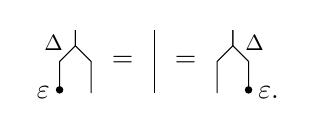
\begin{tikzpicture}[scale=.2]
\draw (-4,0)--(-4,2)--(-5,3)--(-5,4);
\draw (-6,0)--(-6,2)--(-5,3)--(-5,4);
\node [left, scale=.8] at (-5.3,3.2) {$\Delta$};
\draw [fill] (-6,.2) circle [radius=.2];
\node [left] at (-6,0) {$\varepsilon$};

\node at (-2,2) {=};
\draw (0,0)--(0,4);
\node at (2,2) {=};

\draw (4,0)--(4,2)--(5,3)--(5,4);
\draw (6,0)--(6,2)--(5,3)--(5,4);
\node [right, scale=.8] at (5.3,3.2) {$\Delta$};
\draw [fill] (6,.2) circle [radius=.2];
\node [right] at (6,0) {$\varepsilon$.};
\end{tikzpicture}
\end{equation*}
Notice that for any chain complex $C$, operad morphisms from $\Uleft(\A)$ to $\End_C$ correspond to counital coalgebra structures on $C$.

Let $\chains(S^1)$ be the cellular chains on the standard model of the circle
\begin{equation*}
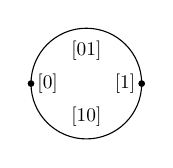
\begin{tikzpicture}
\draw (0,0) circle (20pt);
\node[scale=.7] at (0,12pt){$[01]$};
\node[scale=.7] at (0,-12pt){$[10]$};
\node[scale=.7] at (-14pt,0){$[0]$};
\node[scale=.7] at (14pt,0){$[1]$};
\draw [fill] (-20pt,0) circle [radius=1pt];
\draw [fill] (20pt,0) circle [radius=1pt];
\end{tikzpicture}
\end{equation*}
equipped with a free $\S^\op_2$-action induced by the antipodal map, and let $\chains(S^0)$ be its subcomplex generated by $[0]$ and $[1]$.
We regard these complexes as $\S$-bimodules concentrated in biarity $(2,1)$.

Let $\varphi \colon \chains(S^0) \to \A$ be define by sending $[0]$ and $[1]$ respectively to
\begin{equation*}
	\begin{tikzpicture}[scale=.2]
	\draw (-4,0)--(-4,4);
	\draw (-6,0)--(-6,4);
	\draw [fill] (-6,.2) circle [radius=.2];
	\node [left] at (-6,0) {$\varepsilon$};
	
	\node at (0,.4) {and};
	
	\draw (4,0)--(4,4);
	\draw (6,0)--(6,4);
	\draw [fill] (6,.2) circle [radius=.2];
	\node [right] at (6,0) {$\varepsilon$.};
	\end{tikzpicture}
\end{equation*}

Consider the push-out
\begin{equation*}
\begin{tikzcd}
F(\chains(S^0)) \arrow[r, "F(\varphi)"] \arrow[d] & \A \arrow[d, dashed] \\
F(\chains(S^1)) \arrow[r, dashed] & \mu \vee \A. \\
\end{tikzcd}
\end{equation*}
We think of $\mu \vee \mathcal A$ as the prop obtained by attaching an $\S$-free $1$-cell in biarity $(2,1)$.

Define $\mathcal M$ as the quotient of $\mu \vee \A$ by the ideal generated by
\begin{equation*}
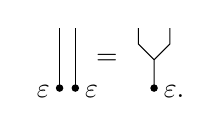
\begin{tikzpicture}[scale=.2]
\draw (0,0)--(0,4);
\draw [fill] (0,.2) circle [radius=.2];
\node [left] at (0,0) {$\varepsilon$};
\draw (1,0)--(1,4);
\draw [fill] (1,.2) circle [radius=.2];
\node [right] at (1,0) {$\varepsilon$};
\node at (3,2) {=};

\draw (5,4)--(5,3)--(6,2)--(6,0);
\draw (7,4)--(7,3)--(6,2);
\draw [fill] (6,.2) circle [radius=.2];
\node [right] at (6,0) {$\varepsilon$.};
\end{tikzpicture}
\end{equation*}